%----------- Pin style
\tikzstyle{every pin edge}=[<-,shorten <=1pt]

%----------- Block style 1
\tikzstyle{neuron}=[draw,circle,fill=black!25,minimum size=17pt,inner sep=0pt]

%----------- Block style 1
\tikzstyle{input neuron}=[neuron, fill=white!80!green, minimum size=1cm]

%----------- Block style 1
\tikzstyle{output neuron}=[neuron, fill=white!80!blue, minimum size=1cm]

%----------- Block style 1
\tikzstyle{hidden neuron}=[neuron, fill=blue!20, minimum size=1cm]

%----------- Block style 1
\tikzstyle{annot} = [text width=4em, text centered]

% Define a distance to separate the layers of the network
\def\layersep{2*2.5cm}

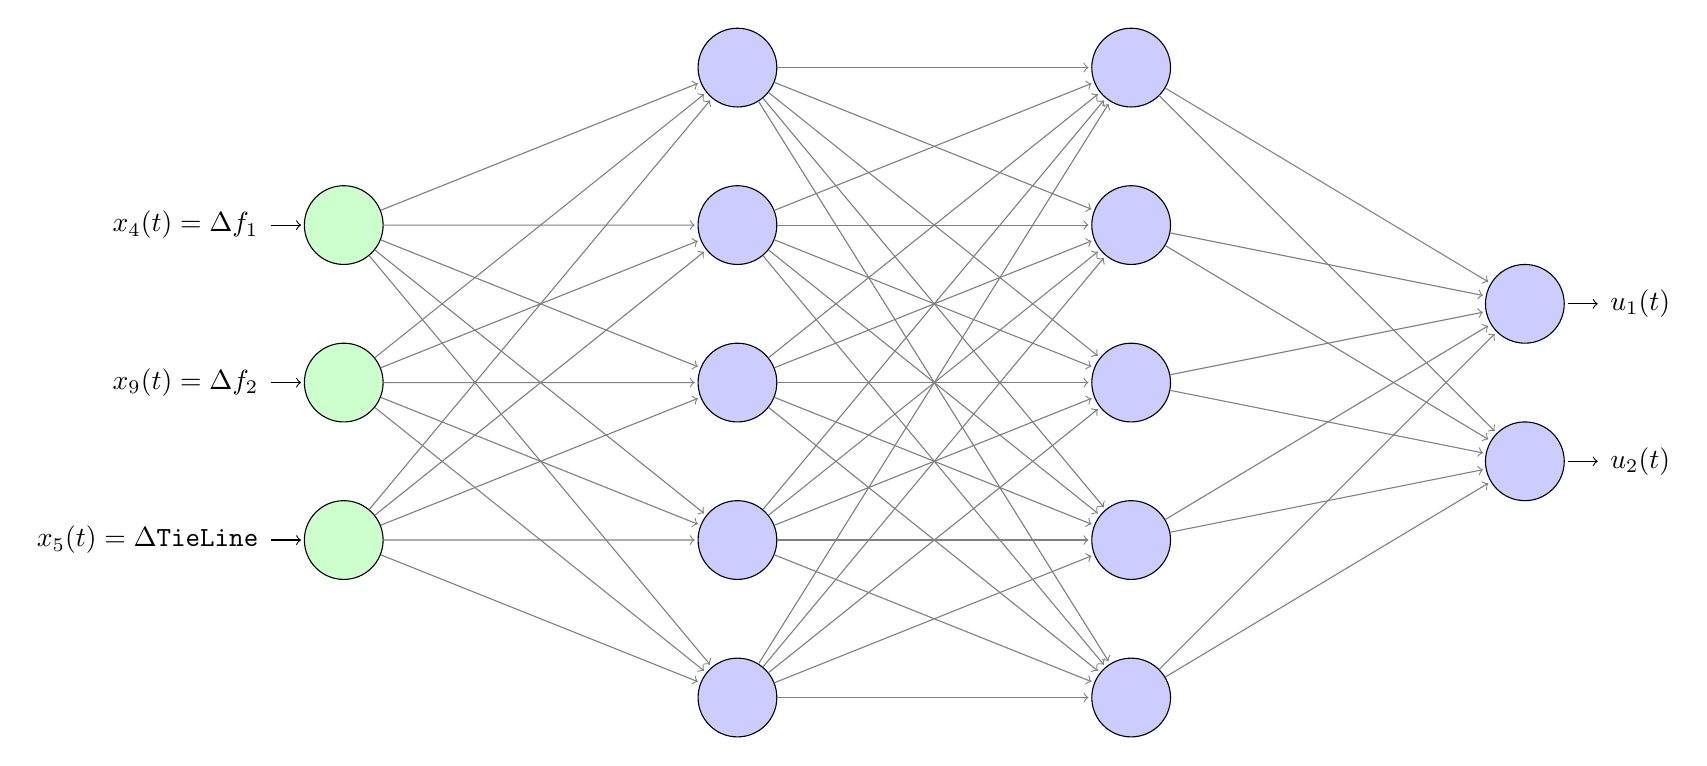
\begin{tikzpicture}[shorten >=1pt,->, node distance=\layersep]
    
    % Draw the input layer nodes
    \foreach \i\y\j in {1/1/$\boldsymbol{x_4(t) = \Delta f_1}$, 2/2/$\boldsymbol{x_9(t) = \Delta f_2}$, 3/3/$\boldsymbol{x_5(t) = \Delta \texttt{TieLine}}$}
    % This is the same as writing \foreach \name / \y in {1/1,2/2,3/3,4/4}
        \node[input neuron, pin=left:\j] (I-\i) at (0,-2*\y) {};

    % Draw the hidden layer 1 nodes
    \foreach \name / \y in {1,...,5}
        \path[yshift=2*1cm]
            node[hidden neuron] (H1-\name) at (\layersep,-2*\y cm) {};
	
	% Draw the hidden layer 2 nodes
	\foreach \name / \y in {1,...,5}
		\path[yshift=2*1cm]
			node[hidden neuron] (H2-\name) at (2*\layersep,-2*\y cm) {};
	
    % Draw the output layer node
    \foreach \name / \y in {1/$\boldsymbol{u_1(t)}$,2/$\boldsymbol{u_2(t)}$}
    	\path[yshift=-2*0.5cm]
    		node[output neuron, pin={[pin edge={->}]right:\y}] (O-\name) at (3*\layersep,-2*\name cm) {};

    % Connect every node in the input layer with every node in the
    % hidden layer 1.
    \foreach \source in {1,...,3}
        \foreach \dest in {1,...,5}
            \path (I-\source) edge [color=gray] (H1-\dest);
	
	% Connect every node in hidden layer 1 with every node in
	% hidden layer 2.
	\foreach \source in {1,...,5}
		\foreach \dest in {1,...,5}
			\path (H1-\source) edge [color=gray] (H2-\dest);
	
    % Connect every node in the hidden layer with the output layer
    \foreach \source in {1,...,5}
    	\foreach \dest in {1,...,2}
        	\path (H2-\source) edge [color=gray] (O-\dest);
    
\end{tikzpicture}